\documentclass[../main.tex]{subfiles}

\begin{document}

\section{Results}

Before commenting the execution times, we will point out the problem domain:
\begin{itemize}
    \item Grid size: 100, 1000, 2000.
    \item Iterations: 100, 1000, 10000, 100000.
    \item \acrshort{mpi} workers: 1, 2, 4, 8, 16, 32.
    \item \acrshort{omp} threads: 4.
\end{itemize}

Since we want to know the scalability of our problem with \acrshort{mpi}, we have locked the number of \acrshort{omp} threads to 4, because in the last assignment it had some of the best results, and we will be able to compare our baseline (4/1 threads/worker) with the rest of the results.

We will do a comparison of the raw execution times between the hybrid implementations and its serial counterparts in \textit{Figure \ref{fig:mpi-serial-exec}}.

\begin{figure}[!htb]
    \centering
    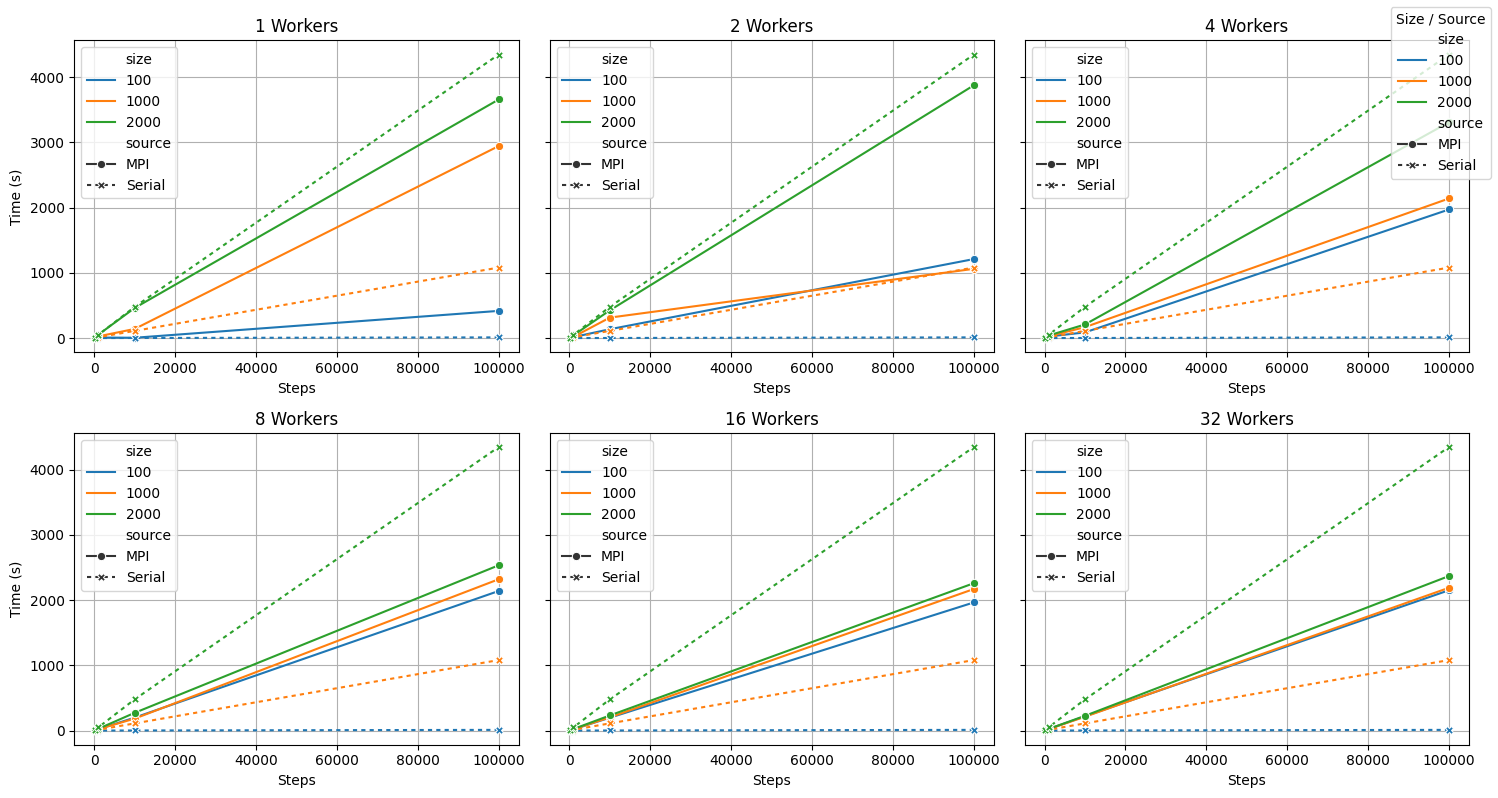
\includegraphics[width=\linewidth]{\subfix{../../media/figures/mpi-serial-comparison.png}}\
    \caption{Time results of the executions}
    \label{fig:mpi-serial-exec}
\end{figure}

With these times and the following formulas, we can calculate the speedups in \textit{Figure \ref{fig:mpi-speedup}} and \textit{Figure \ref{fig:mpi-speedup-size}}, by comparing the execution time of the \acrshort{mpi} baseline, and with \textit{N} workers as in \textit{Formula \ref{formula:speedup}}.

\begin{equation}
    \begin{split}
        Speedup&=\frac{T_{1x4}}{T_{N_{MPI\_ranks}}x4}
    \end{split}
    \label{formula:speedup}
\end{equation}

\begin{figure}[!htb]
    \centering
    \label{fig:mpi-speedups}
    \begin{subfigure}{0.49\textwidth} 
        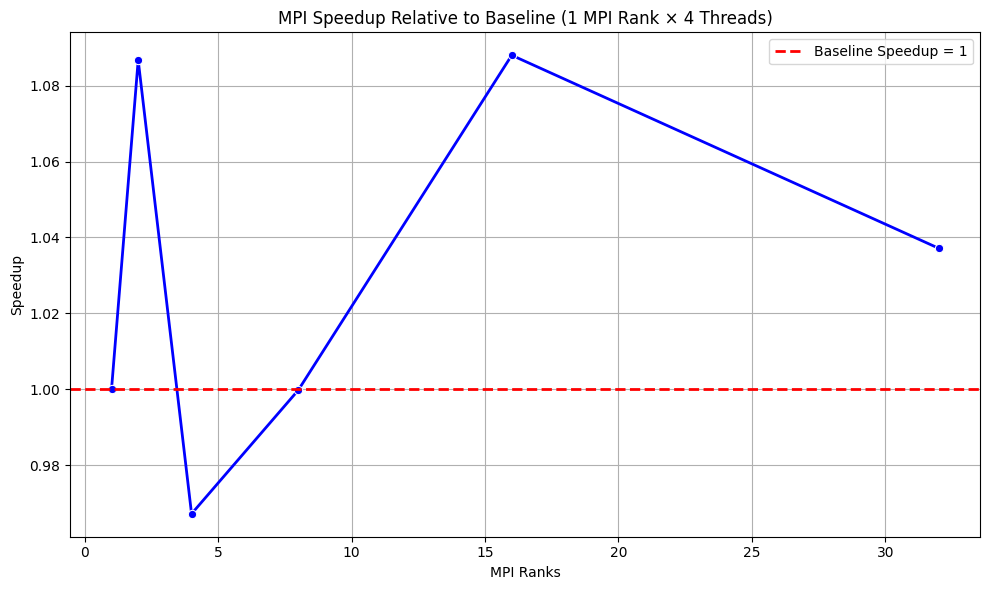
\includegraphics[width=0.8\linewidth]{\subfix{../../media/figures/mpi-speedup-baseline.png}}
        \caption{Speedup compared with baseline}
        \label{fig:mpi-speedup}
    \end{subfigure}
    \begin{subfigure}{0.49\textwidth}
         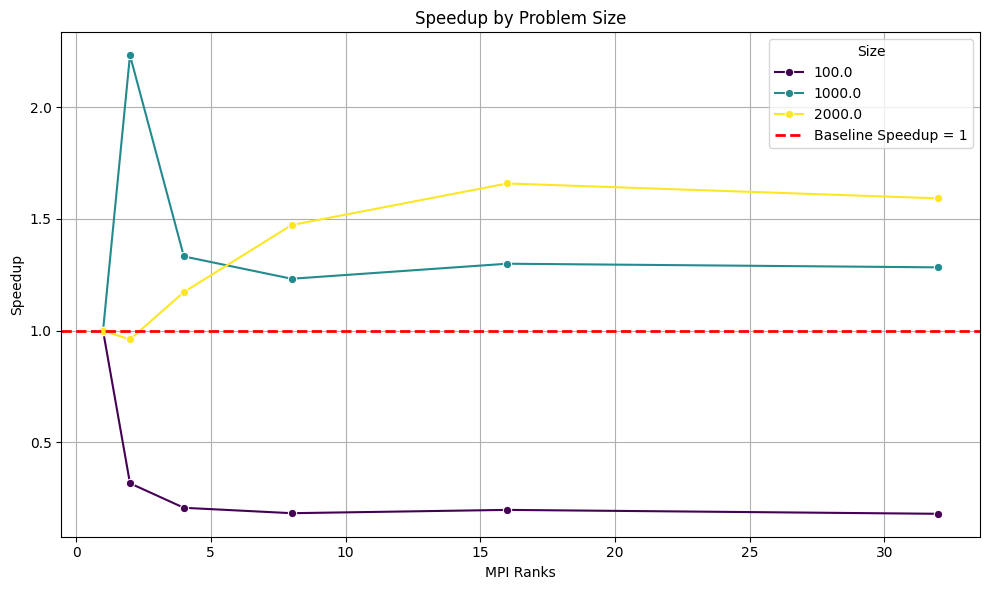
\includegraphics[width=0.8\linewidth]{\subfix{../../media/figures/speedup-size.png}}
        \caption{Speedup compared with baseline by problem size}
        \label{fig:mpi-speedup-size}
    \end{subfigure}
\end{figure}

With speedups calculated, we can also calculate the efficiency and the overhead. To do so, we will use \textit{Formula \ref{formula:total-cores}}, \textit{Formula \ref{formula:efficiency}} and \textit{Formula \ref{formula:overhead}}.
Begin $T_{ideal}$ the baseline time divided by the number of cores.

\begin{equation}
    \begin{split}
        Total\ cores&= N_{MPI\_ranks} x 4
    \end{split}
    \label{formula:total-cores}
\end{equation}
\begin{equation}
    \begin{split}
        Effiency&=\frac{Speedup}{Total\ cores}
    \end{split}
    \label{formula:efficiency}
\end{equation}
\begin{equation}
    \begin{split}
        Overhead(percentage)&=(1\textminus\frac{T_{ideal}}{T_P}) x 100
    \end{split}
    \label{formula:overhead}
\end{equation}

And having as result these metrics in \textit{Figure \ref{fig:mpi-efficiency}} and \textit{Figure \ref{fig:mpi-overhead}}, and by problem size \textit{Figure \ref{fig:mpi-efficiency-size}} and \textit{Figure \ref{fig:mpi-overhead-size}}.


\begin{figure}[!htb]
    \centering
    \label{fig:mpi}
    \begin{subfigure}{0.49\textwidth}
        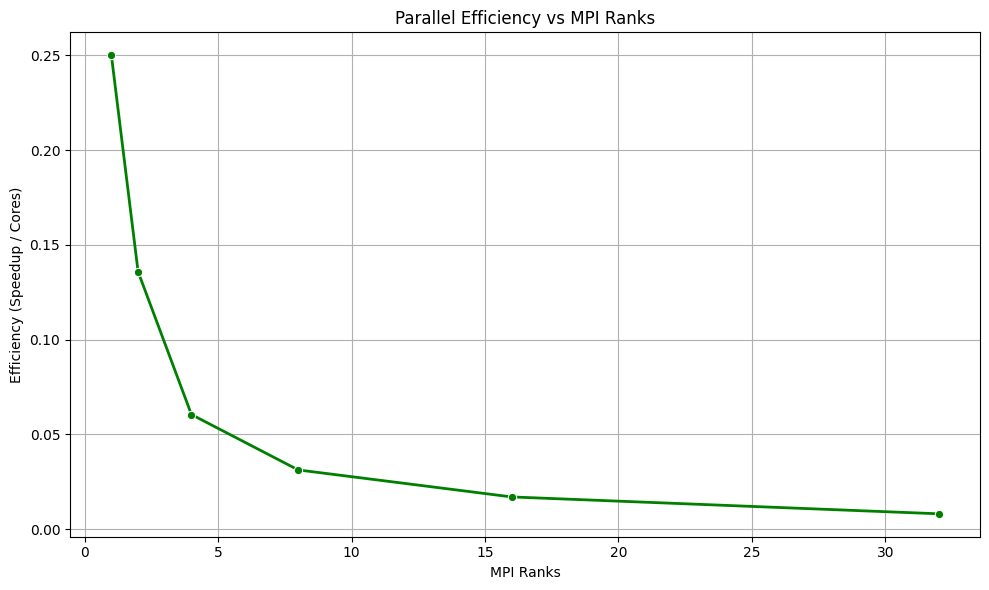
\includegraphics[width=0.8\linewidth]{\subfix{../../media/figures/efficiency.png}}
        \caption{Efficiency of the number of nodes}
        \label{fig:mpi-efficiency}
    \end{subfigure}
    \begin{subfigure}{0.49\textwidth}
        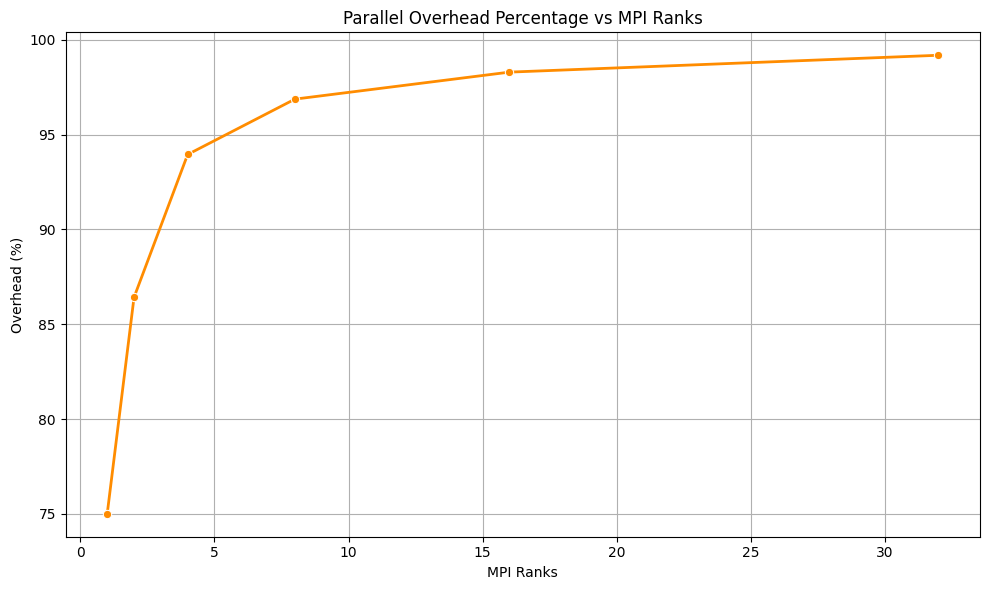
\includegraphics[width=0.8\linewidth]{\subfix{../../media/figures/overhead.png}}
        \caption{Overhead of the communications}
        \label{fig:mpi-overhead}
    \end{subfigure}
\end{figure}

\begin{figure}[!htb]
    \centering
    \label{fig:mpi-size}
    \begin{subfigure}{0.49\textwidth}
        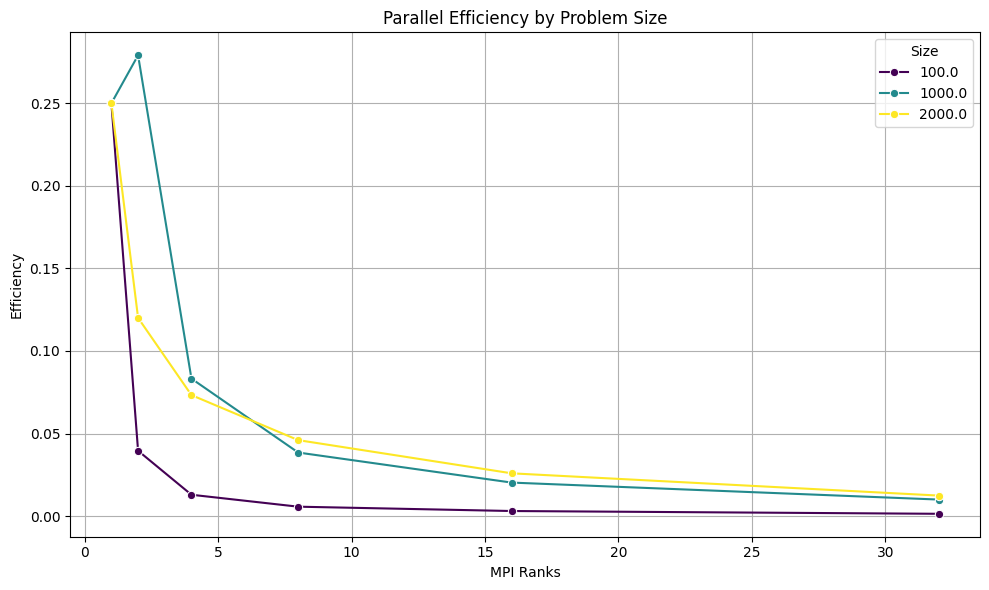
\includegraphics[width=0.8\linewidth]{\subfix{../../media/figures/efficiency-size.png}}
        \caption{Efficiency of the number of nodes by problem size}
        \label{fig:mpi-efficiency-size}
    \end{subfigure}
    \begin{subfigure}{0.49\textwidth}
        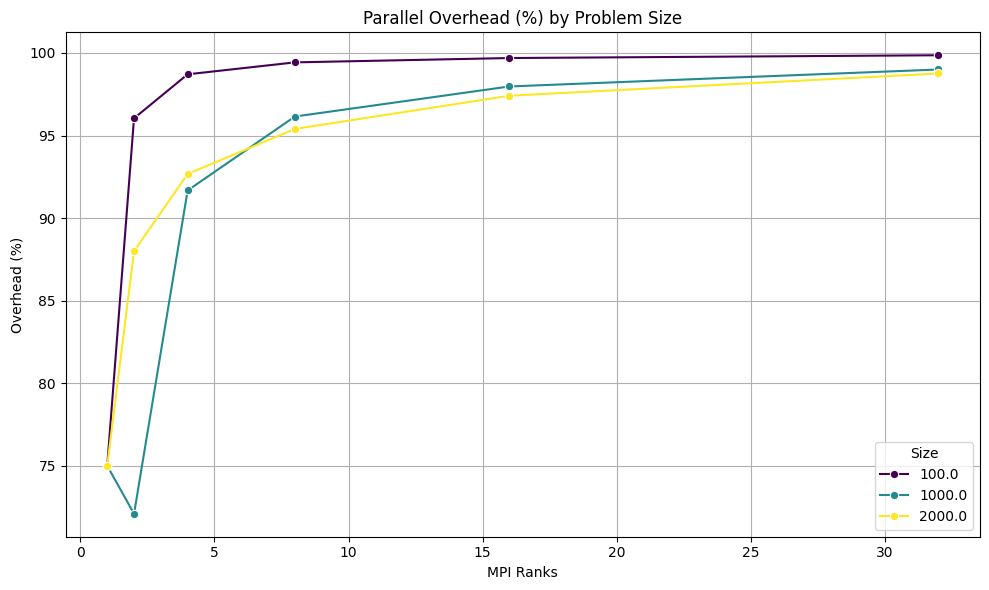
\includegraphics[width=0.8\linewidth]{\subfix{../../media/figures/overhead-size.png}}
        \caption{Overhead of the communications by problem size}
        \label{fig:mpi-overhead-size}
    \end{subfigure}
\end{figure}


\end{document}